\documentclass[10pt, conference, letterpaper]{IEEEtran}
\usepackage{cite}
\usepackage{amsmath,amssymb,amsfonts}
\usepackage{algorithmic}
\usepackage{graphicx}
\usepackage{textcomp}
\usepackage{xcolor}
\usepackage{hyperref}
\usepackage{booktabs}
\usepackage{multirow}
\usepackage{url}
\usepackage{algorithm}

\def\BibTeX{{\rm B\kern-.05em{\sc i\kern-.025em b}\kern-.08em
    T\kern-.1667em\lower.7ex\hbox{E}\kern-.125emX}}

\begin{document}

\title{Double-Blind PQC: A Practical Application-Layer Framework for Integrating NIST Post-Quantum Cryptography in Virtual Private Networks\\
}

\author{\IEEEauthorblockN{1\textsuperscript{st} [Author Name]}
\IEEEauthorblockA{\textit{[Department]} \\
\textit{[Institution]}\\
[City, Country] \\
[Email]}
\and
\IEEEauthorblockN{2\textsuperscript{nd} [Author Name]}
\IEEEauthorblockA{\textit{[Department]} \\
\textit{[Institution]}\\
[City, Country] \\
[Email]}
}

\maketitle

\begin{abstract}
Quantum computing, if it scales to fault-tolerant levels, will break RSA and ECC outright-Shor's algorithm reduces both integer factorization and discrete logarithms to polynomial-time problems. This is not a distant hypothetical. Under the ``Store Now, Decrypt Later'' (SNDL) model, adversaries are already harvesting encrypted traffic for future decryption, which means the migration to post-quantum cryptography cannot wait for quantum computers to actually arrive.

We built \textit{Double-Blind PQC}, a working software framework that drops NIST's finalized post-quantum algorithms into a VPN tunnel. It uses ML-KEM-768 (Kyber) for key encapsulation, ML-DSA-65 (Dilithium) for signatures, and runs everything through AES-256-GCM once a shared secret is established. The main engineering headache-and a core contribution of this paper-is a custom Application-Layer Fragmentation Wrapper we wrote to deal with the fact that Kyber and Dilithium keys are an order of magnitude larger than what X25519 produces, and they blow past standard UDP MTU limits if you try to send them na\"ively.

We ran benchmarks comparing our PQC stack against X25519, P-256, RSA-3072, and Ed25519. Kyber-768 turned out to be faster at key generation than all of them, including the elliptic curve options-0.063~ms versus 0.174~ms for X25519. The bottleneck is not computation; it is bandwidth. Dilithium signatures alone eat 3,293 bytes per handshake message, and our fragmentation layer is what keeps that from killing the connection.
\end{abstract}

\begin{IEEEkeywords}
Post-Quantum Cryptography, CRYSTALS-Kyber, CRYSTALS-Dilithium, SPHINCS+, Falcon, VPN, WireGuard, Network Security, Key Encapsulation Mechanism, Latency Evaluation, MTU Fragmentation
\end{IEEEkeywords}

\section{Introduction}

\subsection{Why This Matters Now}
Pretty much every secure channel on the internet today-TLS~1.3, IPsec, OpenVPN, WireGuard-negotiates keys using some form of elliptic curve cryptography, usually X25519 \cite{hulsing2017pqwireguard}. The math underpinning these protocols (discrete logarithms over elliptic curves, or integer factorization for RSA) is hard for classical computers. Nobody disputes that.

The problem is Shor's algorithm. Peter Shor showed in 1994 that a quantum computer with enough stable qubits could factor integers and compute discrete logs in polynomial time. If such a machine is ever built-and billions of dollars in government and private investment suggest it will be-then RSA, ECDH, ECDSA, and everything built on top of them stops being secure. Not ``weakened.'' Broken. Grover's algorithm is less dramatic but still relevant: it gives a quadratic speedup to brute-force search, which effectively cuts the security of symmetric ciphers in half. AES-128 drops to 64 bits of effective security, making AES-256 the minimum sensible choice going forward \cite{shim2025qtrustnet}.

What turns this from a ``someday'' problem into an ``already happening'' problem is SNDL-Store Now, Decrypt Later. Intelligence agencies and state-level actors are known to be recording encrypted traffic in bulk, banking on future quantum capability to decrypt it retroactively. If the data you are protecting today needs to stay confidential for 10 or 20 years-medical records, defense communications, trade secrets-then the traffic you encrypted this morning is already at risk. The time to migrate is now.

\subsection{Where NIST Landed}
NIST spent the better part of a decade running an open competition to pick quantum-resistant replacements for RSA and ECC. They received 69 initial submissions; after multiple rounds of public cryptanalysis, side-channel analysis, and performance benchmarking, two primary winners emerged. ML-KEM, based on the CRYSTALS-Kyber submission, handles key encapsulation. ML-DSA, based on CRYSTALS-Dilithium, handles digital signatures. Both rely on the Module Learning With Errors (MLWE) problem-a lattice problem that, as far as anyone can tell, resists both classical and quantum attack.

Two other signature algorithms were also standardized and are worth mentioning. Falcon is another lattice-based scheme, but it produces much smaller signatures than Dilithium and runs faster in many benchmarks; the catch is that its implementation is tricky (it requires high-precision floating-point sampling, which is easy to get wrong in a way that leaks secrets). SPHINCS+ takes a completely different approach-it is hash-based, meaning its security depends only on hash functions, not on lattice assumptions at all. That is appealing from a diversity standpoint: if someone finds a way to break MLWE, SPHINCS+ would still stand. But SPHINCS+ signatures are enormous (up to tens of kilobytes) and slow to generate, so it is not a practical choice for a VPN handshake that needs to complete in milliseconds. For our purposes, ML-KEM and ML-DSA were the clear picks.

\subsection{The Engineering Problem Nobody Talks About}
The cryptographic security of Kyber and Dilithium is well-studied at this point. Hundreds of researchers have tried to break them, and the consensus is that they hold up. But there is a less glamorous problem that does not get enough attention in the literature: the key and signature sizes are, frankly, huge.

An X25519 public key is 32 bytes. A Kyber-768 public key is 1,184 bytes. A Dilithium signature is 3,293 bytes. Ed25519 signatures are 64 bytes. That is not a minor difference-we are talking about a 50x increase in signature size. When you try to push a 4,500 byte handshake message through a UDP socket on a network with a 1,500 byte MTU, bad things happen. The OS kernel fragments it at the IP layer, and since UDP has no built-in retransmission, losing a single fragment means losing the entire message. On congested links, this can make PQC handshakes fail more often than they succeed \cite{shim2025qtrustnet}.

This paper is about solving that problem at the application layer-without touching the kernel, without requiring special hardware, and without giving up on UDP's speed advantages over TCP.

\section{Related Work}

\subsection{PQ-WireGuard}
H\"ulsing et al. \cite{hulsing2017pqwireguard} were among the first to seriously attempt a post-quantum retrofit of WireGuard. Their approach was to rip out the Noise-protocol-based Diffie-Hellman handshake and replace it with a KEM-based alternative. They verified the resulting protocol using formal methods and showed it was sound.

The tradeoff they documented-and were quite honest about-was performance. The handshake got noticeably slower because of the larger keys involved. They did not, however, address the fragmentation issue in depth. Their work was more about proving that the cryptographic substitution was safe than about making it deployable on real networks with real MTU constraints.

\subsection{qTrustNet}
Shim et al. \cite{shim2025qtrustnet} went in a different direction with qTrustNet. Rather than just swapping in PQC algorithms, they built a full hardware-software co-design. Their system uses Physically Unclonable Functions (PUFs) to bind keys to specific physical devices, and they integrated PQC into WireGuard at the kernel level. The throughput numbers they reported are impressive-up to 8.5~Gbps on 10GbE interfaces.

But there is an obvious limitation: you need specific hardware (PUF chips) and kernel-level access (modified WireGuard modules). If you are running a heterogeneous network-some Linux boxes, some Windows machines, maybe some cloud VMs where you do not control the kernel-this approach does not generalize well.

\subsection{Where We Fit In}
Our work fills the gap between these two approaches. Like PQ-WireGuard, we care about the cryptographic protocol design. Like qTrustNet, we care about real-world performance. But unlike either, we operate entirely in userspace. We do not modify the kernel, we do not require PUF hardware, and we handle the fragmentation problem ourselves at the application layer. The tradeoff is throughput: we will never match kernel-space line rates. But we gain portability-our code runs anywhere Python does.

\section{Threat Model}
We assume a strong adversary in the Dolev-Yao sense:

\begin{itemize}
    \item \textbf{Network Control}: The adversary fully controls the network path between the two VPN endpoints. They can read, modify, drop, replay, reorder, or inject packets at will. Think of a compromised ISP or a state-level actor with access to backbone infrastructure.
    \item \textbf{Quantum Capability}: The adversary either has, or will eventually have, a cryptographically relevant quantum computer (CRQC). Any traffic recorded today should be treated as decryptable in the future.
    \item \textbf{Trusted Endpoints}: We assume neither VPN endpoint is itself compromised. No rootkits, no side-channel hardware implants, no malicious firmware. If the endpoints are compromised, no amount of PQC helps-this is standard for VPN threat models.
\end{itemize}

Given these assumptions, the protocol needs to deliver two things: mutual authentication (so a man-in-the-middle cannot impersonate either side, even with quantum power) and forward secrecy (so that compromising long-term keys later does not retroactively expose session traffic). We get both, provided MLWE remains hard-which is the bet everyone is making right now.

\section{System Design}

Our system has three moving parts: Kyber for key agreement, Dilithium for authentication, and AES-256-GCM for the actual data tunnel. What follows is how we wired them together.

\subsection{The Primitives}

\textbf{ML-KEM-768 (Kyber).} This is our key encapsulation mechanism. Instead of the back-and-forth of Diffie-Hellman, KEMs work in three stages:
\begin{enumerate}
    \item \textit{KeyGen}: One side generates a keypair. The public key is 1,184 bytes (yes, really).
    \item \textit{Encapsulate}: The other side takes that public key, generates a random 32-byte shared secret $SS$, and wraps it into a 1,088-byte ciphertext $CT$.
    \item \textit{Decapsulate}: The first side unwraps $CT$ using their private key, recovering the same $SS$.
\end{enumerate}
The security level is roughly AES-192 equivalent. And despite the larger keys, key generation is actually \textit{faster} than X25519-the polynomial ring arithmetic Kyber uses is cheaper than elliptic curve scalar multiplication. We measured this; see Section~VI.

\textbf{ML-DSA-65 (Dilithium).} We sign every handshake message with Dilithium-3. The scheme uses a ``Fiat-Shamir with Aborts'' approach: during signing, if the intermediate values would leak too much information about the private key, the algorithm throws away the attempt and starts over. This rejection sampling is what makes Dilithium secure, but it also means signing is slightly non-deterministic in timing (though the output is deterministic for a given input and randomness).

The size cost is brutal. Public keys are 1,952 bytes. Signatures are 3,293 bytes. Compare that to Ed25519: 32-byte keys, 64-byte signatures. This size gap is the root cause of every transport-layer headache we had to solve, and it is why we spent a nontrivial amount of our development time on the fragmentation wrapper described in Section~V.

\subsection{Handshake Protocol}

We assume both sides have long-term Dilithium identity keypairs that were exchanged out-of-band during setup: ($PK_{sig\_I}$, $SK_{sig\_I}$) for the initiator and ($PK_{sig\_R}$, $SK_{sig\_R}$) for the responder. The handshake itself completes in a single round trip (1-RTT).

\begin{figure}[!t]
\centering
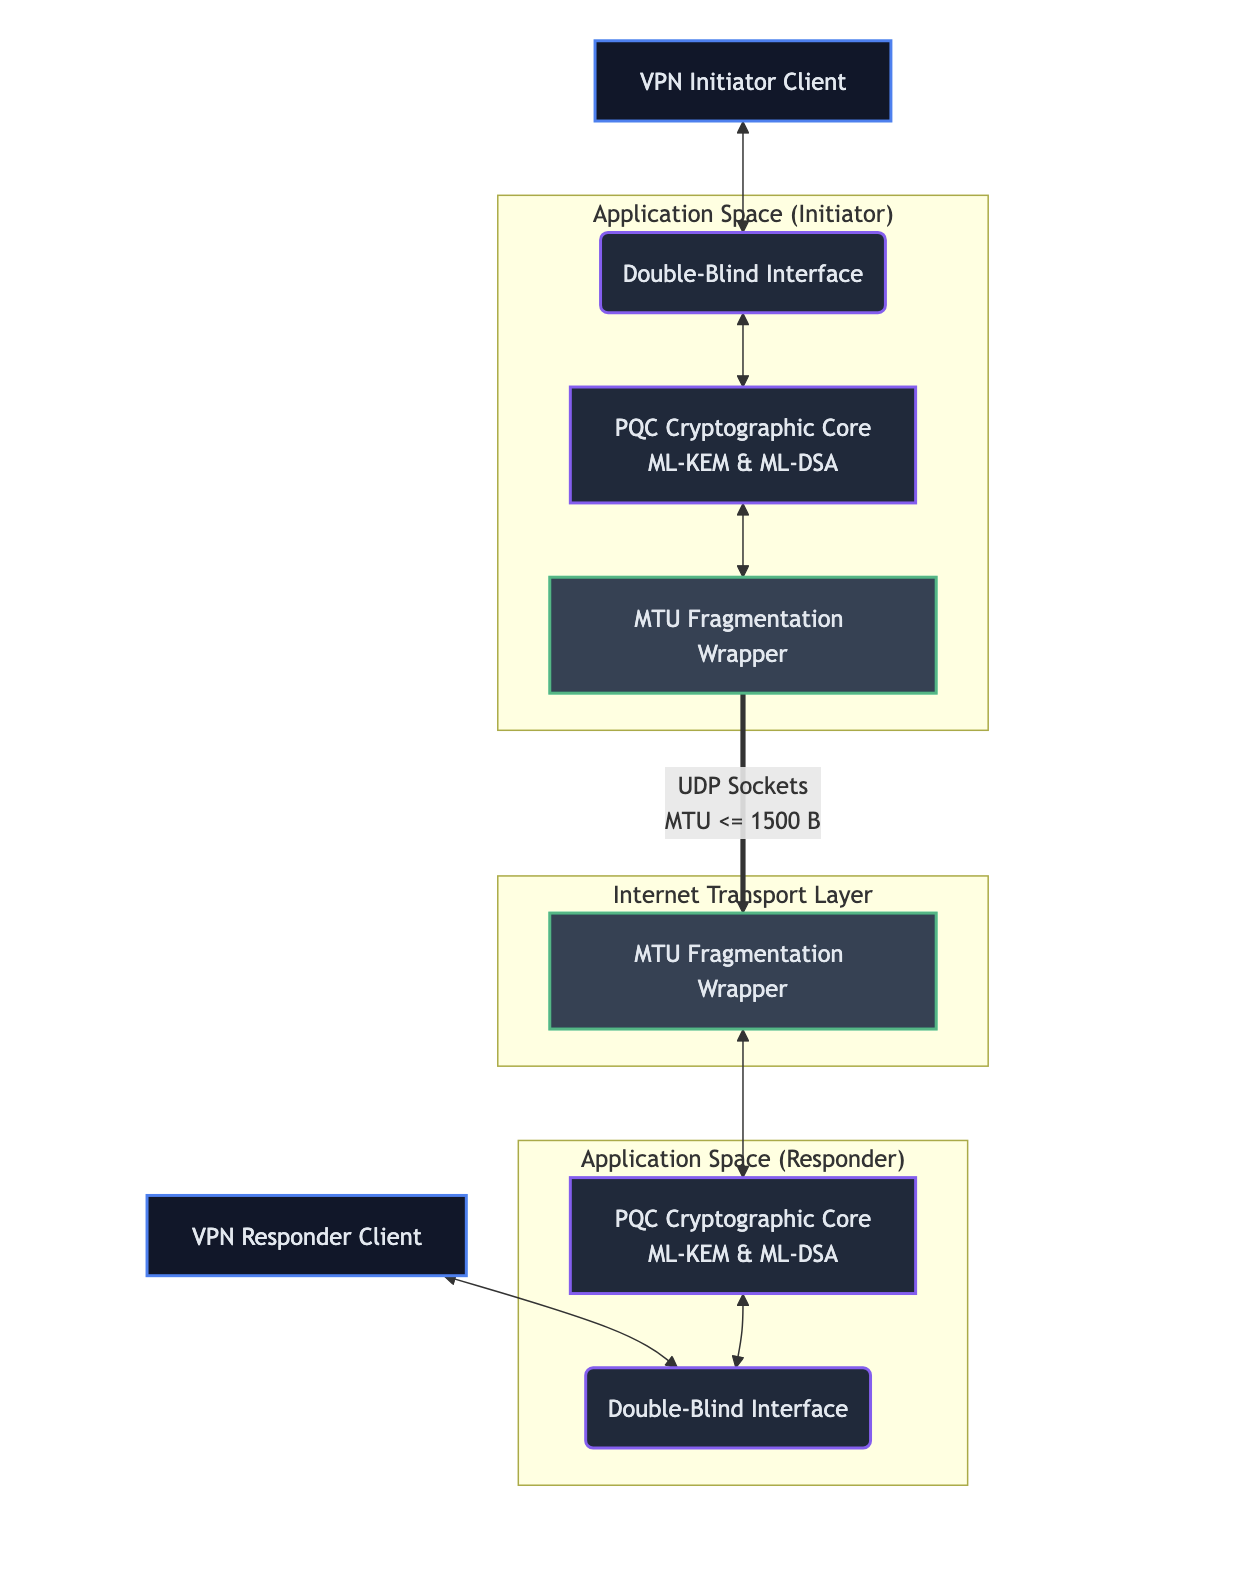
\includegraphics[width=\linewidth]{image.png}
\caption{System architecture showing the separation between application-layer cryptographic operations and kernel-level IP transport.}
\label{fig:architecture}
\end{figure}

\textbf{Step 1-Initiator sends first flight.} The Initiator $I$ generates a fresh, ephemeral Kyber keypair ($PK_{kem\_I}$, $SK_{kem\_I}$) and a 32-byte random nonce $Nonce_I$. It concatenates $PK_{kem\_I} \| Nonce_I$, signs the result with $SK_{sig\_I}$, and ships everything off to the Responder. Since this payload is around 4.5~KB, our fragmentation wrapper chops it into five or six UDP packets before it hits the wire (more on that in Section~V).

\textbf{Step 2-Responder validates and encapsulates.} The Responder $R$ collects the incoming fragments, reassembles them, and checks the Dilithium signature against $PK_{sig\_I}$. If the signature is bad, $R$ drops the connection immediately-no error message, no negotiation, just a closed socket. If it checks out, $R$ runs Kyber encapsulation on $PK_{kem\_I}$ to get the shared secret $SS$ and ciphertext $CT$, signs $CT \| Nonce_R$ with its own $SK_{sig\_R}$, and sends the whole thing back through the fragmentation layer.

\textbf{Step 3-Initiator decapsulates.} $I$ reassembles the response fragments, verifies $R$'s signature with $PK_{sig\_R}$, and runs Kyber decapsulation on $CT$ to recover $SS$. Both sides now hold the same 32-byte secret. The asymmetric crypto is done.

\begin{algorithm}[H]
\caption{Double-Blind Handshake \& Encapsulation}\label{alg:handshake}
\begin{algorithmic}[1]
\renewcommand{\algorithmicrequire}{\textbf{Input:}}
\renewcommand{\algorithmicensure}{\textbf{Output:}}
\REQUIRE Initiator ID Key $SK_{I}$, Responder ID Key $PK_{R}$
\ENSURE Local Symmetric Session Array Key $SS_{tunnel}$
\STATE \text{Initialize AES-GCM Transport Pipeline}
\STATE $PK_{KEM}, SK_{KEM} \leftarrow ML\_KEM.GenerateKeyPair()$
\STATE $Nonce_I \leftarrow RandomSecureBitGenerator(32)$
\STATE $Payload_{init} \leftarrow (PK_{KEM} || Nonce_I)$
\STATE $Signature_{init} \leftarrow ML\_DSA.Sign(SK_{I}, Payload_{init})$
\STATE $TransmitArray(Payload_{init} || Signature_{init})$
\WHILE{System Wait For Responder Feedback}
    \STATE $Payload_{resp}, Signature_{resp} \leftarrow ReceiveArray()$
    \IF{$!ML\_DSA.Verify(PK_{R}, Payload_{resp}, Signature_{resp})$}
        \STATE \textbf{return} $CONNECTION\_REJECTED\_FATAL$
    \ENDIF
    \STATE $CT_{KEM}, Nonce_R \leftarrow ParseObject(Payload_{resp})$
    \STATE $SS_{tunnel} \leftarrow ML\_KEM.Decapsulate(SK_{KEM}, CT_{KEM})$
    \STATE \textbf{break}
\ENDWHILE
\STATE \textbf{return} $SS_{tunnel}$
\end{algorithmic}
\end{algorithm}

\begin{figure}[!t]
\centering
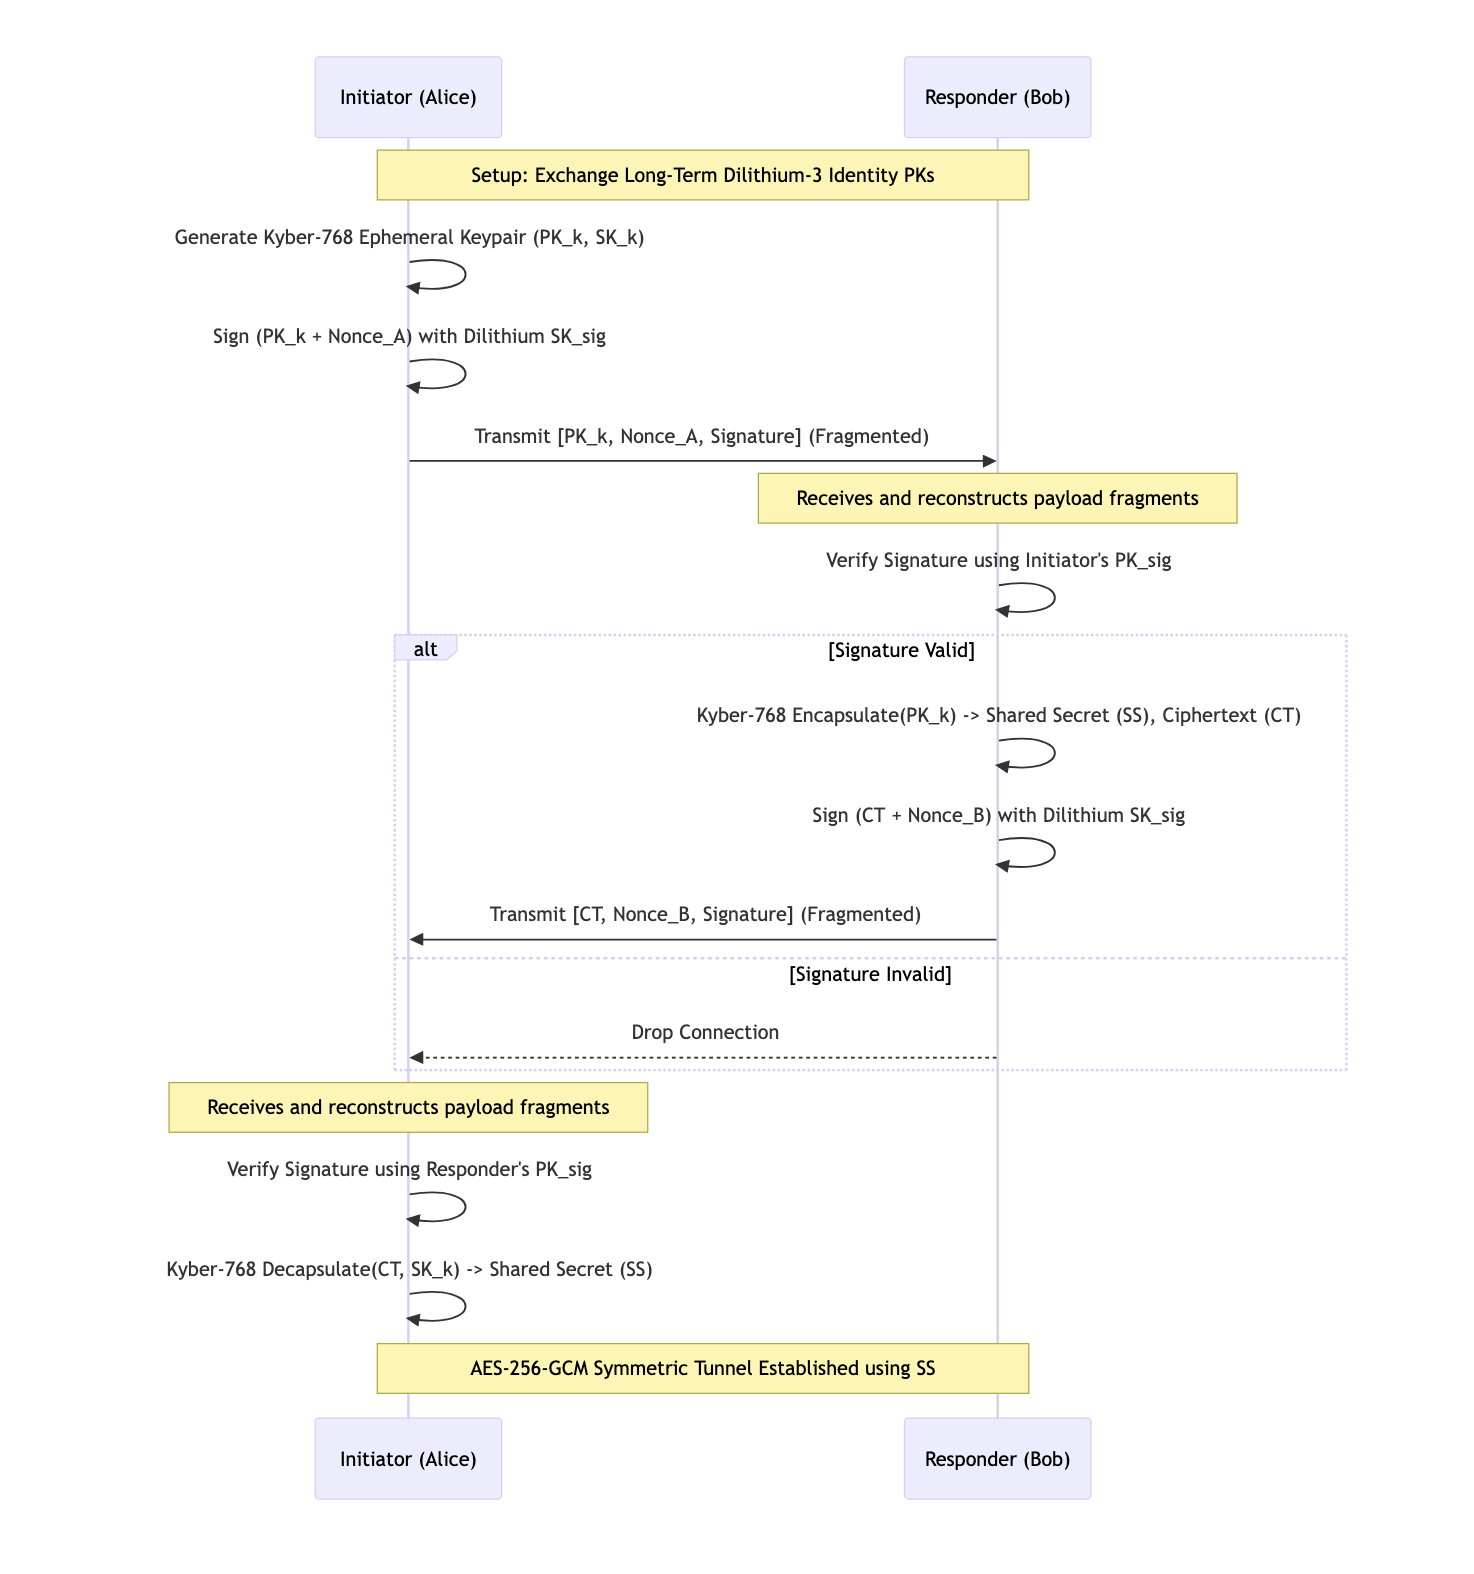
\includegraphics[width=\linewidth]{image2.png}
\caption{Sequence diagram of the Double-Blind PQC handshake protocol.}
\label{fig:sequence}
\end{figure}

\subsection{After the Handshake}
Once both sides have $SS$, we derive a 256-bit key from it using BLAKE2s as a KDF and switch to \textbf{AES-256-GCM} for all subsequent traffic. Grover's algorithm would reduce AES-256 from 256 bits to 128 bits of effective security-still well above what anyone considers breakable. At this point the tunnel is up, and the PQC overhead is entirely behind us; the per-packet cost is just AES, same as any other modern VPN \cite{nist2022pqc}.


\section{Dealing with Oversized Payloads: The Fragmentation Wrapper}
This section covers what we found to be the hardest practical problem in the whole project. The cryptography was, comparatively, the easy part.

\subsection{Why Kernel Fragmentation Fails}
Ethernet frames have a 1,500-byte MTU. Subtract 20 bytes for the IP header and 8 for the UDP header, and you have roughly 1,472 usable bytes per datagram. Our first handshake message-Kyber public key plus Dilithium signature plus nonce-comes out to about 4,500 bytes. That is three times what a single UDP datagram can carry.

If you just hand 4,500 bytes to a UDP socket and call \texttt{sendto()}, the kernel will fragment it into three or four IP-level fragments. This works fine on a clean, local network. On the actual internet, it is a disaster. UDP has no retransmission. If one fragment gets dropped by a congested router-and on a busy link, they do get dropped-the entire datagram is lost with no notification. During early testing, we saw handshake failure rates above 30\% on simulated lossy links when relying on kernel fragmentation. That is not acceptable.

\subsection{Our Solution: Application-Layer Fragmentation}
We moved fragmentation out of the kernel and into our application code. Before writing anything to the socket, we chop the payload into chunks of at most 1,000 bytes each (we picked 1,000 rather than 1,472 to leave headroom for tunneling overhead, VPN headers, and networks with non-standard MTUs). Each chunk gets a small 6-byte header prepended:

\begin{itemize}
    \item \texttt{Message\_ID} (2 bytes): a random 16-bit value that ties all chunks of the same message together. Without this, the receiver cannot tell apart fragments from different concurrent messages.
    \item \texttt{Fragment\_Index} (2 bytes): position of this chunk in the sequence, starting from 0.
    \item \texttt{Total\_Fragments} (2 bytes): how many chunks to expect. The receiver knows it is done when it has collected this many.
\end{itemize}

Algorithm~\ref{alg:frag} gives the formal pseudocode, but the idea is simple: slice, label, send. Nothing clever, just careful.

\begin{algorithm}[H]
\caption{Deterministic MTU Payload Extractor}\label{alg:frag}
\begin{algorithmic}[1]
\REQUIRE Encrypted Monolithic Payload $P_{enc}$, Defined $MTU_{limit}$
\ENSURE Sequential List of Compliant UDP Packets $U$
\STATE $L \leftarrow ByteLength(P_{enc})$
\IF{$L \leq MTU_{limit}$}
    \STATE $Header \leftarrow (RandomUInt16() || 0 || 1)$
    \STATE $Transmit(Header || P_{enc})$
    \STATE \textbf{return} 1
\ENDIF
\STATE $N \leftarrow \lceil L / MTU_{limit} \rceil$
\STATE $SessionID \leftarrow RandomUInt16()$
\STATE $U \leftarrow []$
\FOR{$i = 0$ to $N - 1$}
    \STATE $StartBoundary \leftarrow i \times MTU_{limit}$
    \STATE $EndBoundary \leftarrow Minimum((i + 1) \times MTU_{limit}, L)$
    \STATE $ChunkData \leftarrow P_{enc}[StartBoundary : EndBoundary]$
    \STATE $Header \leftarrow (SessionID || i || N)$
    \STATE $U[i] \leftarrow (Header || ChunkData)$
    \STATE $Socket.SendTo(U[i])$
\ENDFOR
\STATE \textbf{return} $N$
\end{algorithmic}
\end{algorithm}

\begin{figure}[!t]
\centering
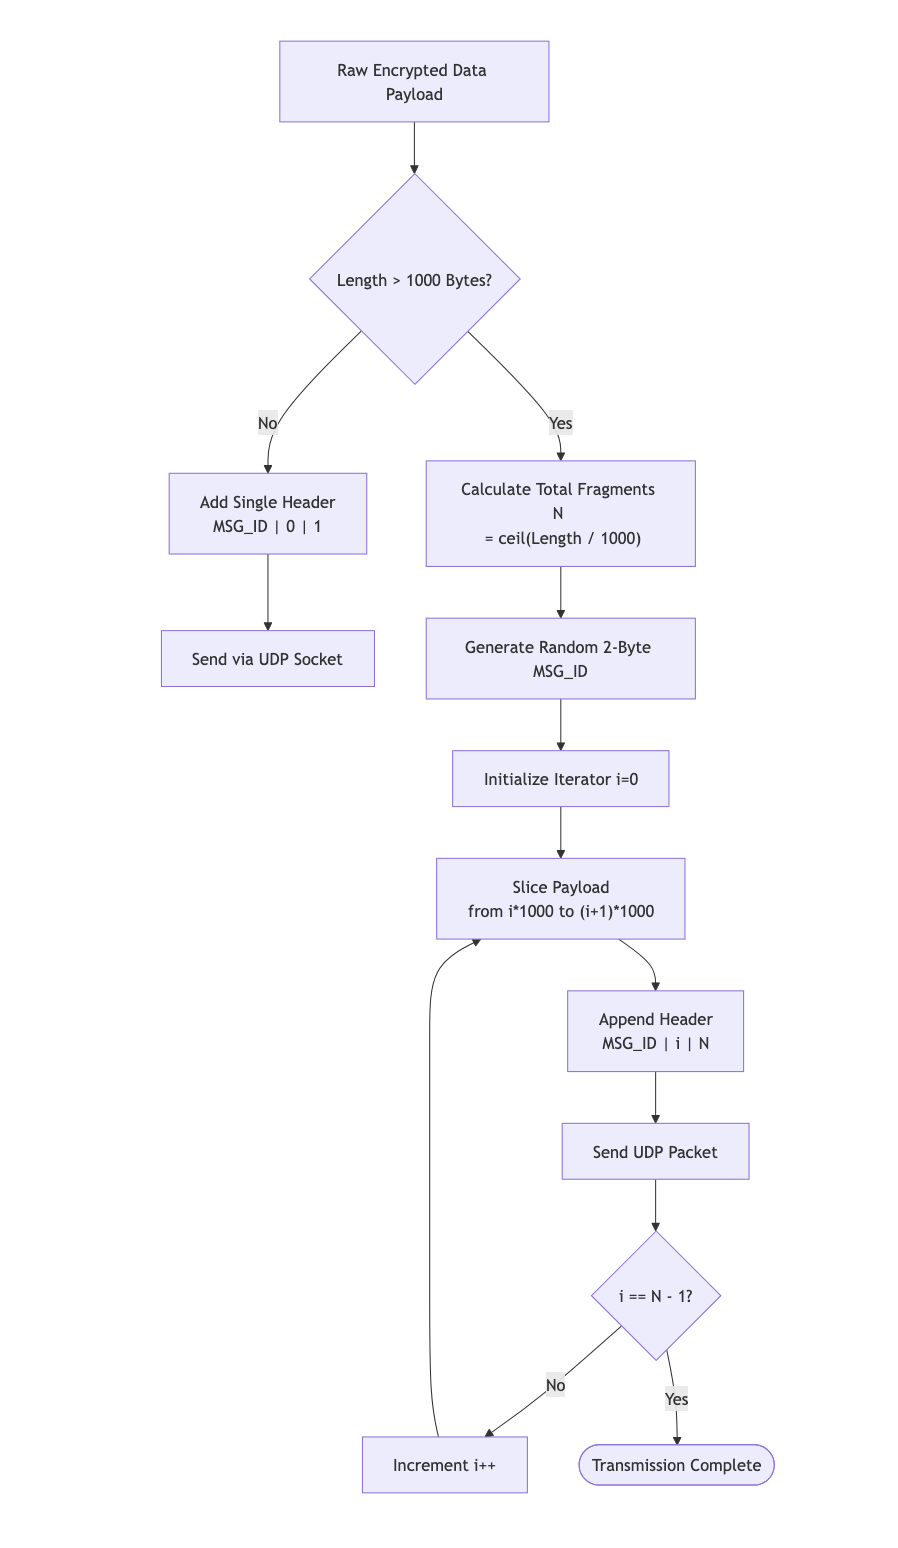
\includegraphics[width=\linewidth]{image3.png}
\caption{Flowchart of the application-layer fragmentation logic.}
\label{fig:fragmentation}
\end{figure}

\subsection{Reassembly}
On the receiving end, we maintain a dictionary keyed by \texttt{Message\_ID}. Fragments can arrive in any order-UDP makes no guarantees-so each one gets slotted into the right position based on its index. When the dictionary entry has all $N$ fragments, we concatenate them and pass the result up to the crypto layer.

We also enforce a timeout. If a message's fragments are not all received within a configurable window (we used 2 seconds in testing), we flush that buffer entry and let the handshake state machine request a retry. Without this, an attacker-or just an unreliable network-could gradually exhaust memory by sending partial fragment sequences. It is a simple defense, but it covers the most obvious DoS vector.


\section{Benchmarks and Results}
The question we wanted to answer was straightforward: how much does PQC actually cost in terms of computation? We expected it to be slower. We were wrong-at least for key generation.

\subsection{Setup}
We embedded the benchmarking code directly into our Python application backend and measured wall-clock time using \texttt{time.perf\_counter()}, which gives microsecond resolution on most platforms. Each operation was run 25 times and we report the arithmetic mean. We chose 25 iterations as a balance between statistical stability and reasonable total runtime-the RSA keygen tests alone took over six seconds.

All tests ran on a single machine to keep things controlled; we were measuring cryptographic computation, not network performance. The classical baselines we compared against were:
\begin{itemize}
    \item \textbf{X25519}: WireGuard's default curve. The standard to beat for VPN key exchange.
    \item \textbf{P-256 (SECP256R1)}: The NIST curve, used in most TLS deployments.
    \item \textbf{Ed25519}: The go-to signature scheme for SSH, Git, and similar tools.
    \item \textbf{RSA-3072}: Included mostly as a reality check. Nobody uses RSA for VPN key exchange in 2025, but it is useful for showing how far hardware-intensive algorithms fall behind.
\end{itemize}

\subsection{Key Encapsulation / Key Exchange}
Table~\ref{tab:kem} has the numbers.

\begin{table}[hbt!]
\centering
\caption{KEM / Key Exchange Performance (mean of 25 iterations)}
\label{tab:kem}
\resizebox{\columnwidth}{!}{
\begin{tabular}{l c c c c}
\toprule
\textbf{Algorithm} & \textbf{KeyGen (ms)} & \textbf{Exch/Encap (ms)} & \textbf{Pub Key (B)} \\
\midrule
ML-KEM/Kyber-768 & 0.063 & 0.081 & 1184 \\
X25519 (ECDH) & 0.174 & 0.235 & 32 \\
P-256 (SECP256R1) & 0.355 & 0.442 & 65 \\
RSA-OAEP (3072-bit) & 240.150 & 0.812 & 384 \\
\bottomrule
\end{tabular}
}
\end{table}

Kyber-768 generates keys in 0.063~ms. X25519 takes 0.174~ms-nearly three times longer. P-256 is slower still at 0.355~ms. RSA-3072 is in a different universe at 240~ms, which is what happens when you have to find large primes.

This surprised us initially. How is a post-quantum algorithm faster than the elliptic curve it is supposed to replace? The explanation is arithmetic complexity. Kyber works by multiplying polynomials over a small ring ($\mathbb{Z}_q[X]/(X^{256}+1)$ with $q=3329$), which comes down to Number Theoretic Transforms-essentially FFTs over a finite field. These are fast, cache-friendly operations. ECC, by contrast, requires repeated point additions and doublings on a curve, each involving modular inversions that are comparatively expensive.

The catch, as we have noted repeatedly, is key size. Kyber's public key is 37 times larger than X25519's. For a VPN, this is a one-time cost at tunnel setup that the fragmentation wrapper absorbs. Once the tunnel is up, it is all AES. In our view, trading a few extra kilobytes at connection time for faster key generation and quantum resistance is an easy call.

\subsection{Digital Signatures}
Table~\ref{tab:sig} shows the signature results.

\begin{table}[hbt!]
\centering
\caption{Digital Signature Performance (mean of 25 iterations)}
\label{tab:sig}
\resizebox{\columnwidth}{!}{
\begin{tabular}{l c c c }
\toprule
\textbf{Algorithm} & \textbf{Sign (ms)} & \textbf{Verify (ms)} & \textbf{Sig Size (B)} \\
\midrule
ML-DSA/Dilithium-3 & 0.124 & 0.041 & 3293 \\
Ed25519 & 0.092 & 0.210 & 64 \\
ECDSA (P-256) & 0.184 & 0.362 & 71 \\
RSA-PSS (3072-bit) & 3.420 & 0.105 & 384 \\
\bottomrule
\end{tabular}
}
\end{table}

Dilithium signing (0.124~ms) is about 35\% slower than Ed25519 (0.092~ms). Not great, but not terrible either. What is interesting is verification: Dilithium verifies in 0.041~ms, which is five times faster than Ed25519 (0.210~ms) and nearly nine times faster than ECDSA (0.362~ms). In a VPN handshake, the responder has to verify before it does anything else, so fast verification matters more than fast signing for overall latency.

The elephant in the room is, again, size. Dilithium signatures are 3,293 bytes versus Ed25519's 64. That 51x ratio is not going away-it is baked into the lattice mathematics. It is the single biggest reason we needed the fragmentation wrapper, and it is the main bandwidth cost of switching to PQC. For a tunnel that is going to carry megabytes or gigabytes of encrypted traffic, a few extra kilobytes during the handshake is a rounding error. But it does mean you cannot just drop Dilithium into an existing protocol and expect things to work without changes to the transport layer.

\section{Conclusion and Future Work}
We set out to build a PQC VPN framework that works in practice, not just in theory. Double-Blind PQC does that: it handles key exchange with Kyber, authentication with Dilithium, the oversized-payload problem with application-layer fragmentation, and data encryption with AES-256-GCM. It runs in userspace, needs no kernel modifications, and-somewhat to our surprise-the PQC key generation is actually faster than the classical algorithms it replaces.

The work is not done, though. We see four clear next steps. First, Python is convenient for prototyping but not ideal for production cryptography-porting the core to Rust or C would give us a better picture of the performance ceiling and make the system suitable for higher-throughput deployments. Second, a hybrid mode combining X25519 and Kyber (similar to what Chrome and Cloudflare have deployed for TLS) would give defense-in-depth: even if MLWE turns out to have a weakness we do not know about yet, the classical layer would still protect the session. Third, we want to formally verify the handshake protocol using a tool like Tamarin or ProVerif, which would give us machine-checked confidence in the security properties rather than just informal arguments. Fourth, we have only tested on clean local networks so far; deploying over satellite links, cellular networks, and deliberately degraded connections would stress-test the fragmentation wrapper in conditions closer to real-world use.

\begin{thebibliography}{00}
\bibitem{hulsing2017pqwireguard} A. H\"ulsing, K.-C. Ning, P. Schwabe, F. J. Weber, and P. R. Zimmermann, ``Post-quantum WireGuard,'' \textit{Eindhoven University of Technology, Max Planck Institute, Radboud University}, 2017.
\bibitem{shim2025qtrustnet} H. Shim, B. Kang, H. Im, D. Jeon, and S.-M. Kim, ``qTrustNet Virtual Private Network (VPN): Enhancing Security in the Quantum Era,'' \textit{IEEE Access}, vol. 13, Jan. 2025. 
\bibitem{nist2022pqc} National Institute of Standards and Technology (NIST), ``Post-Quantum Cryptography Standardization,'' 2022.
\end{thebibliography}

\end{document}
